\chapter{\materialsname}

Durante el desarrollo de este documento se han empleado diversas 
herramientas y recursos tecnológicos. Este apartado proporciona una visión clara de las plataformas empleadas, subrayando su importancia para garantizar la trazabilidad y calidad a lo largo del proceso de investigación.

\section{Bases de Datos Científicas} 

La validez de una revisión sistemática depende en gran parte de la legitimidad y cobertura temática 
que ofrecen las fuentes seleccionadas. Este estudio se llevó a cabo mediante la consulta de bases de 
datos científicas de reconocido prestigio:

\begin{table}[H]
\centering
\caption[Bases De Datos Científicas Seleccionadas]{%
    \vspace{4pt}
    \fontsize{9}{11}\selectfont \\
    BASES DE DATOS CIENTÍFICAS SELECCIONADAS \\[2pt] % Tu subtítulo
}
\label{tab:bases_de_datos}
\begin{tabular}{@{} l l @{}}
\hline\hline
\textbf{Base de Datos} & \textbf{Fuente} \\
\hline
Scopus             & https://www.scopus.com \\
IEEE Xplore        & https://ieeexplore.ieee.org \\
ScienceDirect      & https://www.sciencedirect.com \\
Web Of Science     & https://www.webofscience.com \\
\hline\hline
\end{tabular}
\end{table}

\section{Herramientas de Apoyo} 
\subsection{Parsifal}
Esta plataforma web se empleó como herramienta de apoyo metodológico durante la fase de diseño y ejecución de ambas revisiones sistemáticas de la literatura. Su valor radica en que permite estructurar de forma ordenada todo el proceso, desde la definición inicial de los objetivos de investigación hasta la documentación final de los resultados, asegurando en todo momento la trazabilidad y transparencia del trabajo realizado~\cite{ParsifalSite}.

El flujo de trabajo dentro de la herramienta está basado en tres fases principales.

\begin{itemize}
    \item \textbf{Planificación}: incluye la definición del protocolo, la prueba de evaluación de calidad de los articulos y la creación del formulario de extracción de datos.  
    \item \textbf{Ejecución}: comprende la búsqueda bibliográfica, la importación de estudios, el proceso de selección, la evaluación de calidad, la extracción de información y un análisis muy basico realizado de forma automatica por la plataforma de los datos recopilados, genera graficas estandarizadas y de apenas relevancia para la investigación, es una de las principales limitaciones de la plataforma.  
    \item \textbf{Reporte}: en esta fase se sistematizan y presentan los resultados, generando salidas exportables en distintos formatos y listas de referencias.  
\end{itemize}

Cabe destacar que todo el proceso interno se verá de manera detenida en la sección de Metodología, dentro de los apartados correspondientes en las revisiones llevadas a cabo en este trabajo de fin de grado.

A diferencia de alternativas como Rayyan~\cite{RayyanSite} muy empleada en revisiones médicas o Covidence~\cite{CovidenceSite} de carácter comercial y con funcionalidades bajo subscripción, Parsifal ofrece una solución gratuita, accesible vía web y orientada específicamente a revisiones literarias en el ámbito de la ingeniería y la informática.

Todo esto lo convierte en la opción más adecuada, más que incluso el uso de hojas de cálculo tradicionales (Excel o Google Sheets) que requieren un diseño manual de filtros y seguimiento, aumentando el riesgo de inconsistencias.

Otras ventajas destacables son la exportación de datos permitiendo variedad de formatos (CSV, BibTeX), la posibilidad de trabajo colaborativo en línea con múltiples usuarios teniendo un recuento de el trabajo realizado por cada individuo, la identificación de artículos duplicados de forma automática y el guardado en la nube.

No obstante, la plataforma también presenta ciertas limitaciones que son importante considerar. En primer lugar, su conexión con bases de datos externas es bastante restringida, ya que únicamente se encuentra integrada con Scopus y ScienceDirect. Esto reduce la automatización en la importación de resultados procedentes de otras fuentes relevantes como Web of Science o IEEE Xplorer. Asimismo, Parsifal no cuenta con herramientas de análisis cuantitativo avanzado, lo que obligó a complementar este trabajo con el uso de otras herramientas como VOSviewer y Google Colab con Python. Por último, no permite un acceso en modo lectura para terceros, por este motivo, los artículos seleccionados en la fase final se han agrupado en una hoja de Google Sheets, incluida como anexo para facilitar su consulta.\\

A continuación, se muestran una serie de capturas que pretenden ilustrar el flujo de trabajo de la herramienta Parsifal. Estas imágenes demuestran a modo de ejemplo el proceso seguido durante la \hyperref[slr_ciber]{revisión sistemática de la literatura de ciberseguridad en la era post-cuántica}.

El primer paso dentro de la aplicación es crear el protocolo de investigación sobre el cuál girará toda la revisión. \hyperref[metodologia]{La sección de Metodología} de este trabajo describe el protocolo declarado de forma detallada, las siguientes imágenes son tan solo una representación visual de la interfaz con la que se ha trabajado.

\begin{figure}[H]
\centering
\caption[Protocolo de investigación - Parsifal]{
    \vspace{4pt}
    \fontsize{12}{11}\selectfont \\
    Protocolo de investigación - Parsifal\\
}
\footnotesize Fuente: Parfisal
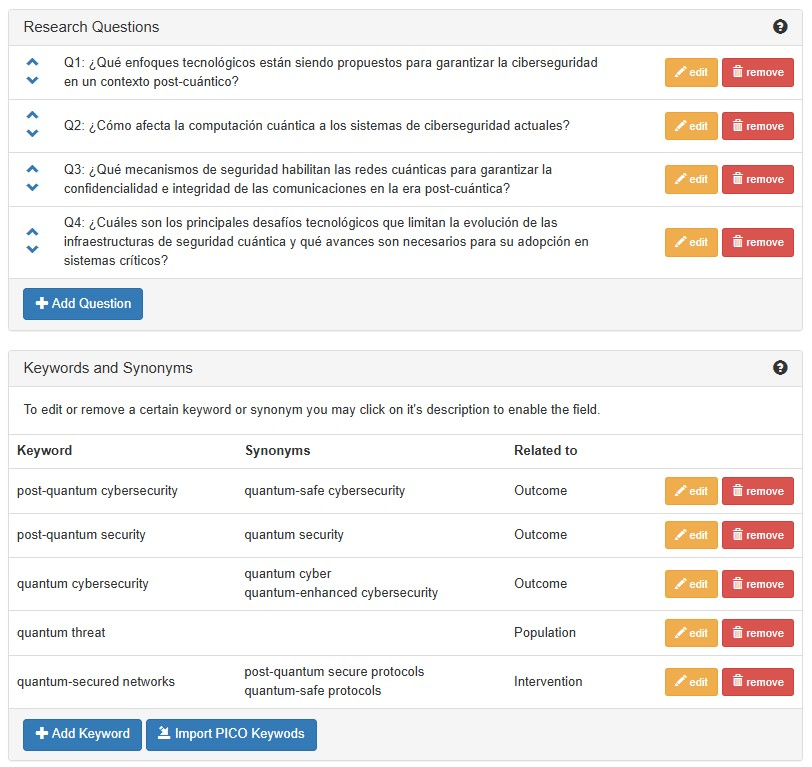
\includegraphics[width=0.90\textwidth]{pictures/Protocolo_parsifal.jpg}
\label{fig:protocolo}
\end{figure}

La búsqueda de estudios en este caso de Scopus funciona ingresando una cadena de búsqueda. La \hyperref[searchString]{cadena de búsqueda} empleada se encuentra adjunta en la sección de Metodología.

\begin{figure}[H]
\centering
\caption[Búsqueda en Scopus - Parsifal]{
    \vspace{4pt}
    \fontsize{12}{11}\selectfont \\
    Búsqueda en Scopus - Parsifal \\
}
\footnotesize Fuente: Parfisal
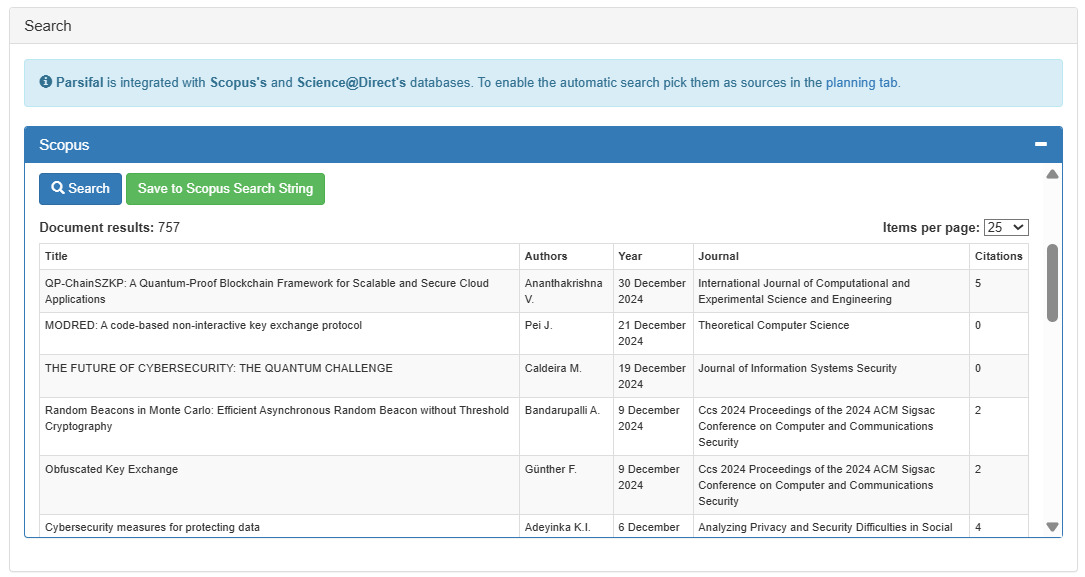
\includegraphics[width=0.90\textwidth]{pictures/SearchScopus_parsifal.jpg}
\label{fig:search_scopus}
\end{figure}

Dado que Parsifal no tiene integración directa con todas las bases de datos empleadas en esta revisión, la herramienta ofrece la posibilidad de importar los estudios.

\begin{figure}[H]
\centering
\caption[Importación de estudios - Parsifal]{
    \vspace{4pt}
    \fontsize{12}{11}\selectfont \\
    Importación de estudios - Parsifal \\
}
\footnotesize Fuente: Parfisal
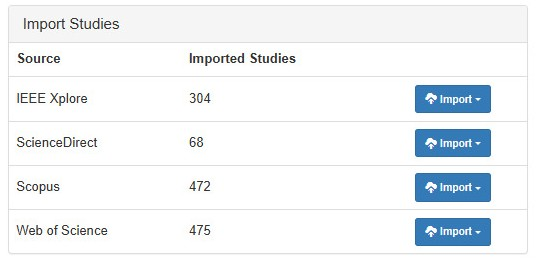
\includegraphics[width=0.90\textwidth]{pictures/ImportStudies_parsifal.jpg}
\label{fig:import_studies}
\end{figure}

Una vez procesados los datos, Parsifal se encargará de mostrar un listado de todos los artículos, cada uno con sus propiedades correspondientes. En la fase de selección de estudios, se revisan detalladamente las propiedades de cada artículos para decidir si son aceptados o no según los \hyperref[criterios]{criterios de inclusión y exclusión} declarados. También en este punto, se identifican y eliminan los artículos duplicados, un problema común al haber realizado búsquedas en múltiples bases de datos.

\begin{figure}[H]
\centering
\caption[Selección de estudios - Parsifal]{
    \vspace{4pt}
    \fontsize{12}{11}\selectfont \\
    Selección de estudios - Parsifal \\
}
\footnotesize Fuente: Parfisal
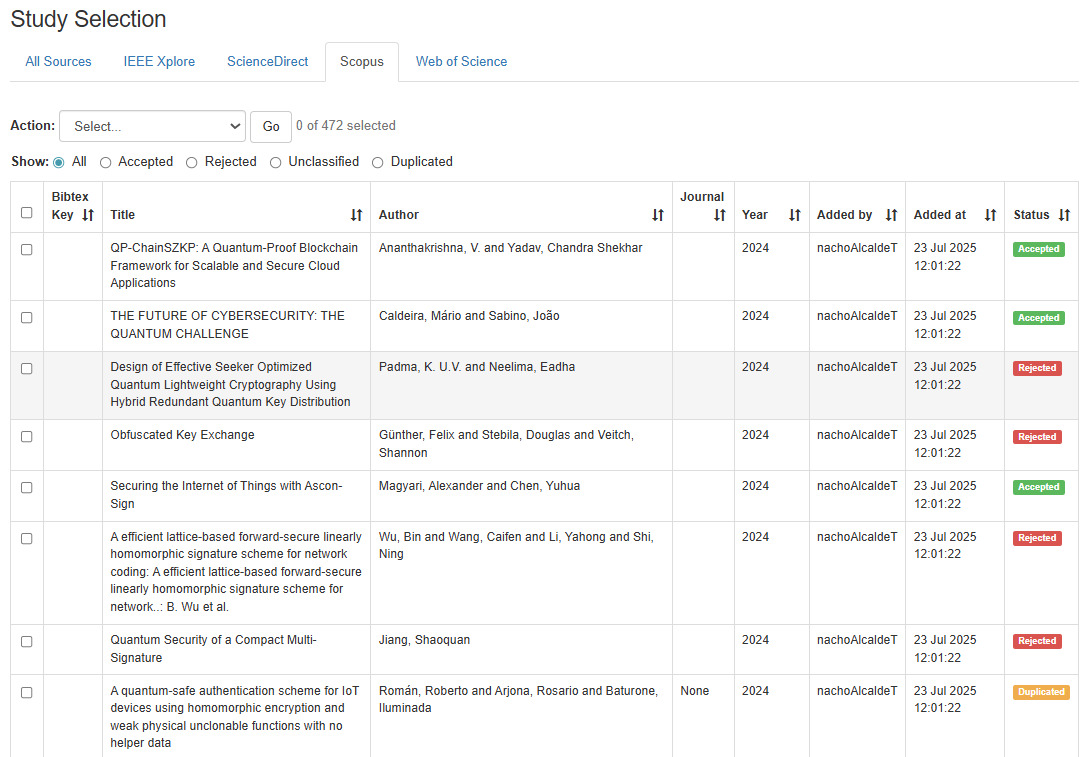
\includegraphics[width=0.90\textwidth]{pictures/StudiesSelection_parsifal.jpg}
\label{fig:studies_selection}
\end{figure}

Asi son mostradas las propiedades de los artículos, tanto el título, la descripción, autores, palabras claves, número de citaciones, facilitando la toma de decisiones en la fase de selección.

\begin{figure}[H]
\centering
\caption[Detalles de los artículos - Parsifal]{
    \vspace{4pt}
    \fontsize{12}{11}\selectfont \\
    Detalles de los artículos - Parsifal \\
}
\footnotesize Fuente: Parfisal
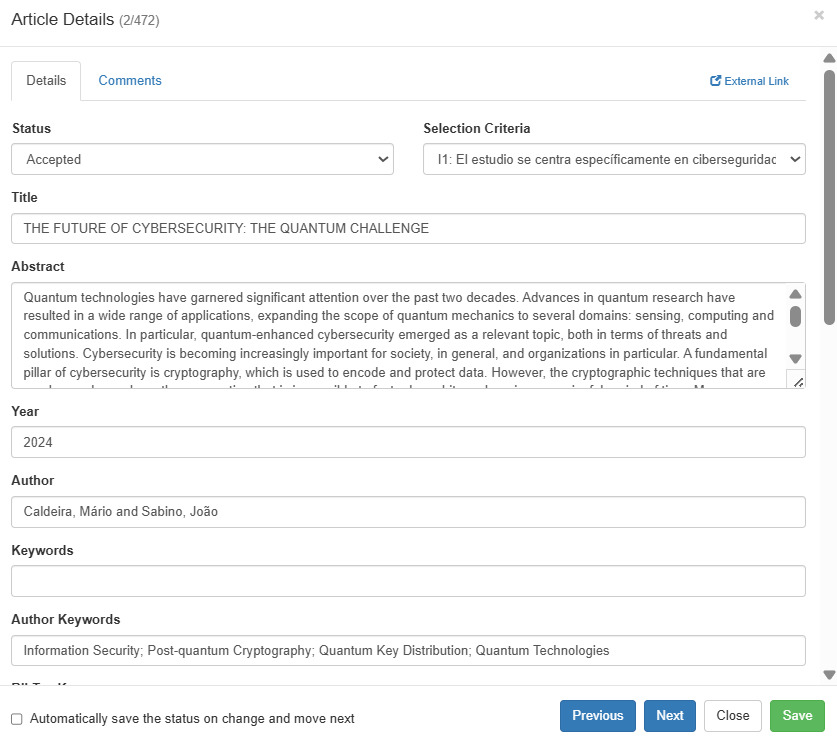
\includegraphics[width=0.90\textwidth]{pictures/articleDetails_parsifal.jpg}
\label{fig:article_details}
\end{figure}

A la sección de evaluación de calidad tan solo acceden aquellos artículos aceptados en la fase previa. Se trata de un segundo filtro donde se evalúa cada trabajo mediante una puntuación, basada en las preguntas de calidad definidas. Solo los artículos que superen una nota mínima de corte serán considerados como parte de la selección final. En esta fase, resulta imprescindible la lectura completa del artículo para poder verificar si cumple con los criterios de calidad establecidos.

\begin{figure}[H]
\centering
\caption[Evaluación de calidad - Parsifal]{
    \vspace{4pt}
    \fontsize{12}{11}\selectfont \\
    Evaluación de calidad - Parsifal \\
}
\footnotesize Fuente: Parfisal
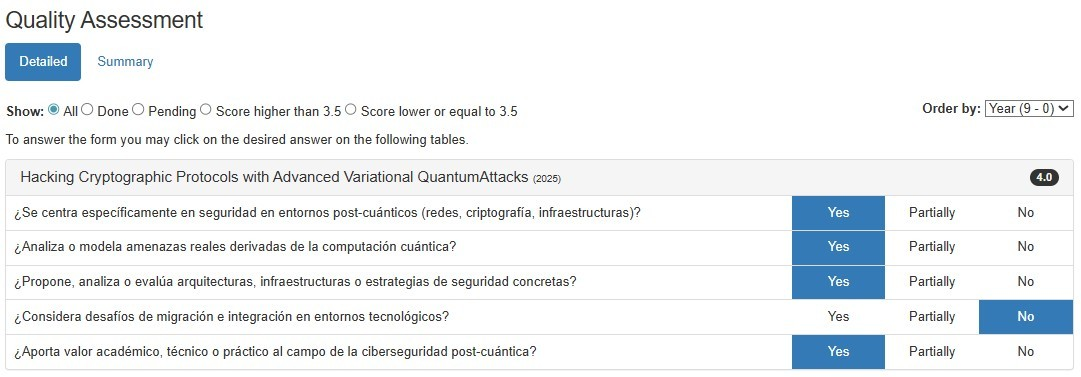
\includegraphics[width=0.90\textwidth]{pictures/qualityAssessments_parsifal.jpg}
\label{fig:quality_assessment}
\end{figure}

Finalmente, la herramienta permite extraer los datos relevantes de los artículos que superaron la evaluación de calidad. Una vez completado, los datos pueden ser descargados, dando por finalizada la revisión.

\begin{figure}[H]
\centering
\caption[Extracción de datos - Parsifal]{
    \vspace{4pt}
    \fontsize{12}{11}\selectfont \\
    Extracción de datos - Parsifal \\
}
\footnotesize Fuente: Parfisal
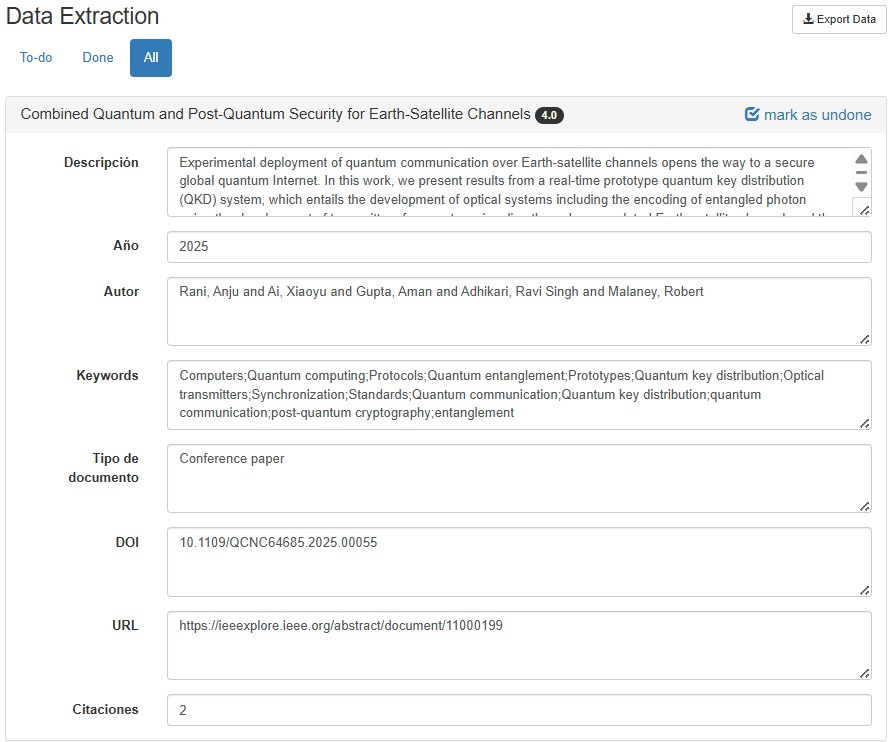
\includegraphics[width=0.85\textwidth]{pictures/dataExtraction_parsifal.jpg}
\label{fig:data_extraction}
\end{figure}

\subsection{VOSviewer}
El análisis y visualización de datos bibliográficos se realizó con VOSviewer, una herramienta especializada en la creación de mapas representativos. Su uso fue clave al permitir identificar patrones, temas emergentes y estructuras temáticas dentro de los campos estudiados. 

La capacidad de generar representaciones gráficas facilitó una comprensión más profunda de los campos de investigación ofrenciendo múltiples funcionalidades que permitieron analizar la literatura desde diferentes perspectivas:

\begin{itemize}
    \item \textbf{Mapas de co-ocurrencia de palabras clave:} representa de forma gráfica qué términos se repiten con mayor frecuencia y cómo se relacionan entre sí. Esta información es útil para validar la cadena de búsqueda y detectar tendencias temáticas emergentes en el conjunto de artículos recuperados.
    
    \item \textbf{Redes de co-citación entre autores o documentos:} identifican autores, artículos o revistas clave en el campo, mostrando cuáles han tenido mayor impacto y cómo se interconectan los estudios.
    
    \item \textbf{Mapas de colaboración institucional y por países:} revelan los grupos de investigación más activos y las relaciones de colaboración a nivel internacional, proporcionando un contexto adicional para interpretar los resultados de la revisión sistemática.
    
    \item \textbf{Opciones de visualización avanzadas:} permite generar clusters, redes, mapas de densidad y mapas de overlay, facilitando la interpretación de información, destacando temas emergentes o evolución temporal.
\end{itemize}

VOSviewer destaca por ser intuitivo, gratuito y ligero lo que facilita su uso para usuarios con poca experiencia en bibliometría. No obstante, su simplicidad también conlleva limitaciones, pues ofrece menos opciones para análisis estadísticos avanzados, comparaciones complejas o personalización detallada de mapas, funcionalidades que sí están presentes en herramientas similares de análisis bibliométrico como CiteSpace~\cite{CiteSpaceSite} o Gephi~\cite{GephiSite}.

En otros contextos, VOSviewer puede aplicarse sobre el conjunto final de artículos, sin embargo, en este trabajo, su uso se limitó a la etapa inicial de exploración para asegurar la construcción adecuada de las cadenas de búsqueda.

A continuación, se presentan dos ejemplos representativos de los mapas generados con VOSviewer:

\begin{figure}[H]
\centering
\caption[Mapa de co-ocurrencia de palabras clave - VOSViewer]{%
    \vspace{4pt}
    \fontsize{12}{11}\selectfont \\
    Mapa de co-ocurrencia de palabras clave - VOSViewer \\ [2pt]
    \footnotesize Fuente: VOSViewer
}
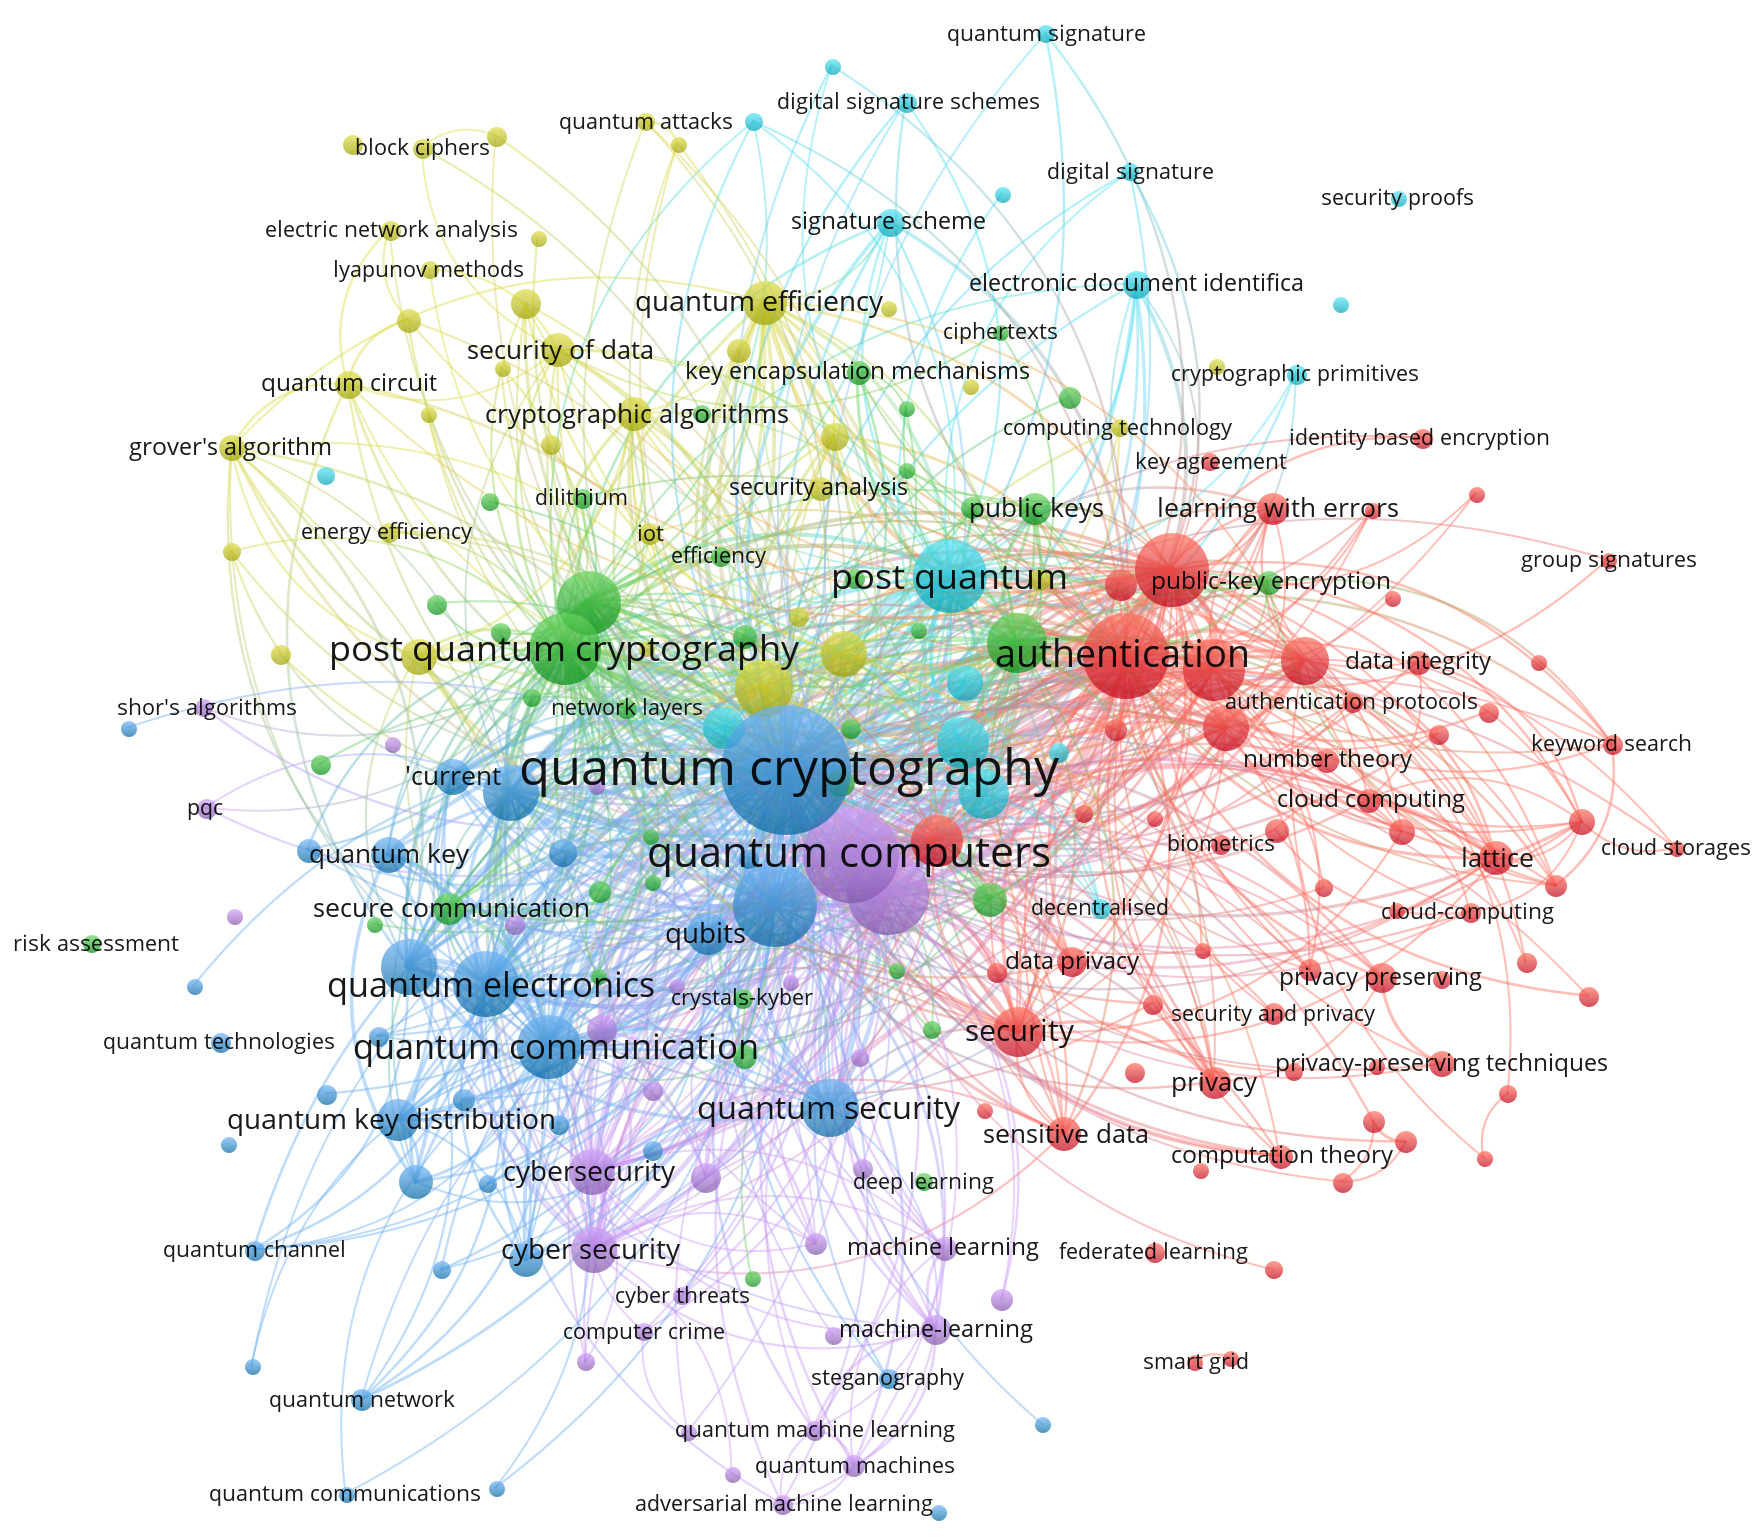
\includegraphics[width=0.93\textwidth]{pictures/ClusteresVosViewer.jpg}
\label{fig:ClusteresVosViewer}
\end{figure}

Este mapa de co-ocurrencia permite visualizar la frecuencia y la relación entre los términos más relevantes. El tamaño de los nodos representan la frecuencia de aparición de las palabras claves, mientras que las conexiones y colores de los clústeres indican las relaciones temáticas y agrupación de conceptos relacionados.

\begin{figure}[H]
\centering
\caption[Red de citaciones - VOSViewer]{%
    \vspace{4pt}
    \fontsize{12}{11}\selectfont \\
    Red de citaciones - VOSViewer\\
}
\footnotesize Fuente: VOSViewer\\
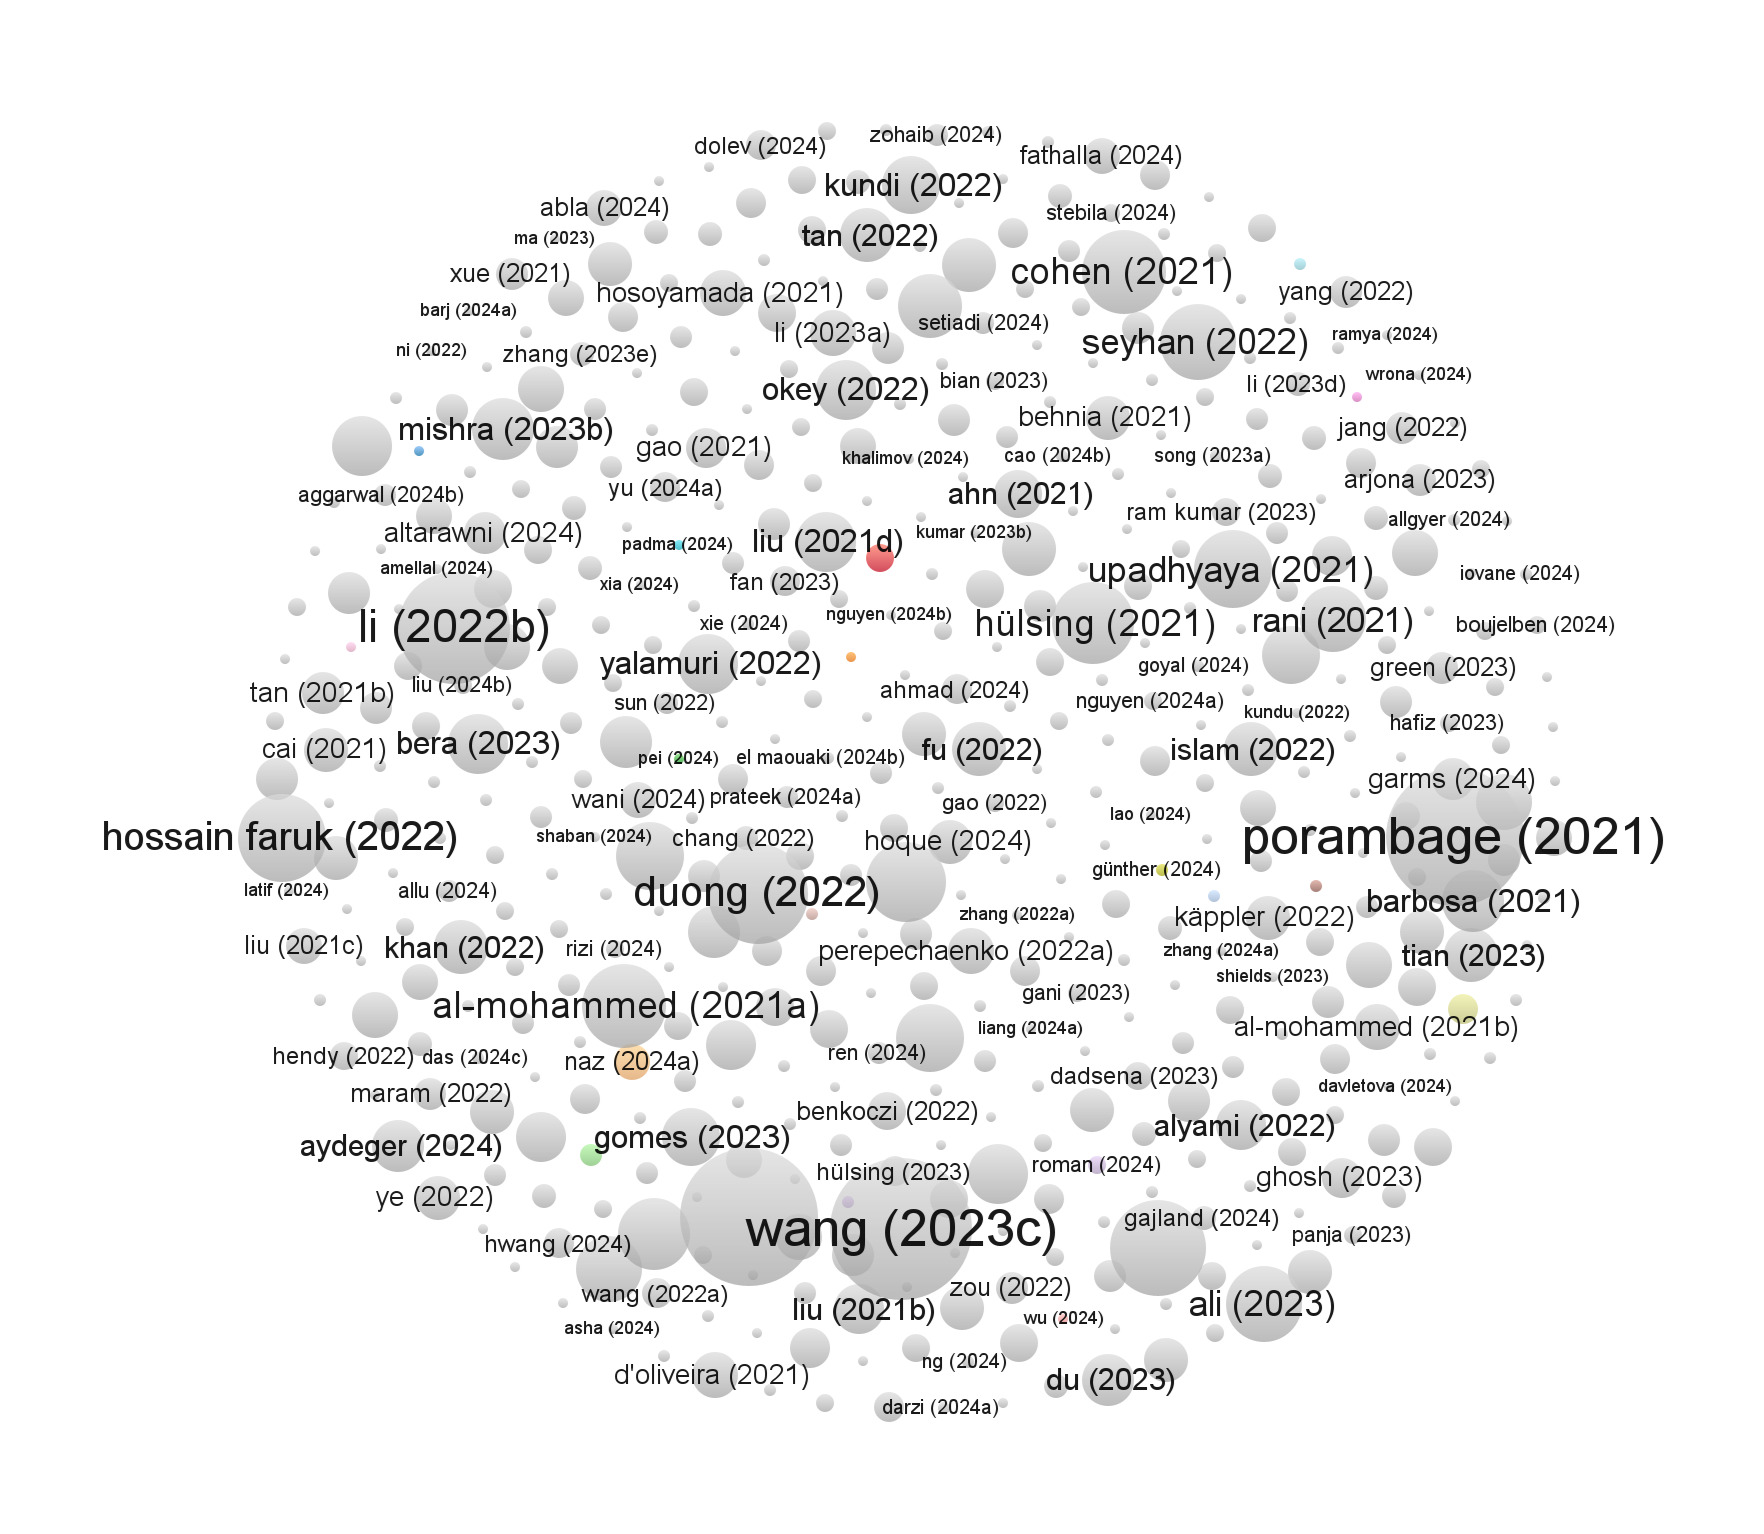
\includegraphics[width=0.93\textwidth]{pictures/CitasVosViewer.jpg}
\label{fig:CitasVosViewer}
\end{figure}

La red de citaciones muestra las conexiones entre los artículos en función de las referencias compartidas. De esta forma, es posible identificar los documentos más influyentes y observar cómo se estructuran los grupos de investigación.


\subsection{Google Colab + Python}
Para el análisis cuantitativo de los artículos finales se utilizó Python dentro del entorno Google Colab. Esta herramienta facilitó el procesamiento eficiente de los datos, permitiendo generar métricas, explorar y visualizar la información bibliográfica recopilada~\cite{GoogleColabSite}.

\begin{figure}[H]
\centering
\begin{minipage}{0.8\textwidth}
    \centering
    {\fontsize{12}{11}\selectfont
     \textbf{Bloque de Código 1} \\
     Librerías utilizadas \\
    }
    \begin{minted}[
        linenos=false,
        frame=single,
        framesep=2mm,
        bgcolor=lightgray!20,
        fontfamily=tt,
        fontsize=\small,
        obeytabs=true,
        tabsize=4
    ]{python}
# Manipulación de los datos bibliográficos y estructuración de tablas.
%pip install pandas

# Generación de visualizaciones como histogramas, gráficos de barras y líneas.
%pip install matplotlib
%pip install seaborn

# Lectura y escritura de archivos Excel, fuente principal de los datos extraídos.
%pip install openpyxl
    \end{minted}
\end{minipage}
\end{figure}

Todo el código utilizado se encuentra disponible a través de los enlaces adjuntos en el anexo de este documento.

\subsection{Canva}
El diseño de las ilustraciones, diagramas y elementos gráficos de este documento han sido diseñadas empleando Canva como herramienta de diseño. Esto facilitó la creación de figuras atractivas y profesionales, asegurando que la gran mayoría de imágenes incluidas fueran de elaboración propia~\cite{CanvaSite}.

\subsection{Overleaf - LaTeX}
La documentación de este trabajo de fin de grado ha sido realizada con la plataforma de escritura científica Overleaf en combinación al lenguaje tipográfico LaTeX. Esta selección permitió mantener en todo momento un formato profesional y consistente a lo largo de este proyecto~\cite{OverleafSite}.

A diferencia de editores tradicionales de texto como Microsoft Word~\cite{MicrosoftWord} o Google Docs~\cite{GoogleDocs}, Overleaf ofrece grandes ventajas que facilitan la organización y control de documentos. Permite la estructuración en carpetas diferenciadas para imágenes, apéndices, secciones, fragmentos de código, pudiendo trabajar individualmente con partes del documento de forma independiente. Asimismo, la plataforma automatiza tareas críticas como referencias, índices, numeración de secciones, páginas y encabezados ahorrando tiempo de edición manual.